\section{PMT Characterization at Room Temperature}
\label{PMTtest}

The PMTs were tested in order to determine their functionality, which was done by the measurement of several parameters. The PMT gain is determined as the mean number of electrons produced by a phototube in response to one photoelectron (PE). The PMT signal (integrated charge spectrum) has been fitted by a sum of an exponential and  a gaussian functions, or, in case of presence of a double photoelectron peak, by a sum of an exponential and two gaussian functions (see Fig.~\ref{figPMTtestSER}). Single PE resolution of a phototube has been calculated as the width ($\sigma$) of the single PE peak, divided by its mean. The `peak-to-valley' ratio is calculated as the ratio of the height of the single PE peak and the valley after the pedestal, and thus quantifies the separation of the noise and signal. These measured quantities characterize the ability to reduce the drift effects of the PMT sensitivity and supply voltage fluctuations, when the tube is operated over extended time periods. 

The facility for PMT testing and characterization has been assembled according to the scheme shown in Fig.~\ref{figPMTtestScheme}. The light tight box with 6 channels provides a possibility to test 5 PMTs simultaneously. During the whole period of the test one PMT has been constantly located in the same spot (channel 5 in the light tight box) and tested in every measurement cycle for calibration purpose, in order to determine possible systematic errors of the measurements. 

\begin{figure}[!ht]
\centering
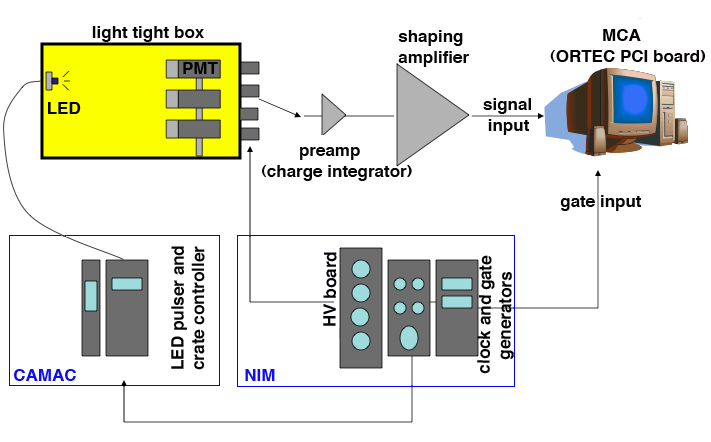
\includegraphics[width=0.8\linewidth]{plots/PMTtest/PMTtestSetupFlip_withLabels.png}
\caption[Schematic diagram of the PMT test facility]{Schematic diagram of the PMT test facility.}
\label{figPMTtestScheme}
\end{figure}

In total, 218 PMTs have been tested. Among them, there are 126 low QE phototubes purchased for the XENON100 detector, 34 low QE PMTs that have been used in the XENON10 experiment, and planned to be installed in XENON100 or kept as spare for possible replacements, and 58 high QE PMTs, with an improved photocathode and QE increased by almost 50\% in average.

The examples of the single PE response measured at room temperature are shown in Fig.~\ref{figPMTtestSER_1} and Fig.~\ref{figPMTtestSER_2}, for one of the PMTs with a good characteristics and considered to be installed in the XENON100 detector, and for one of the PMTs with bad separation between noise and signal and not used in the experiment. Out of 126 low QE PMTs, 4 PMTs did not show a signal, and have been classified as not working and returned to the factory.

\begin{figure}[!t]
\centering
\subfigure[]{
%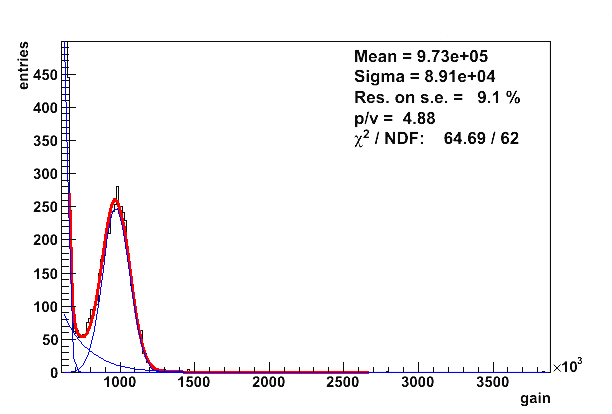
\includegraphics[width=0.475\linewidth]{plots/PMTtest/PMTtest_GoodPMT.png}
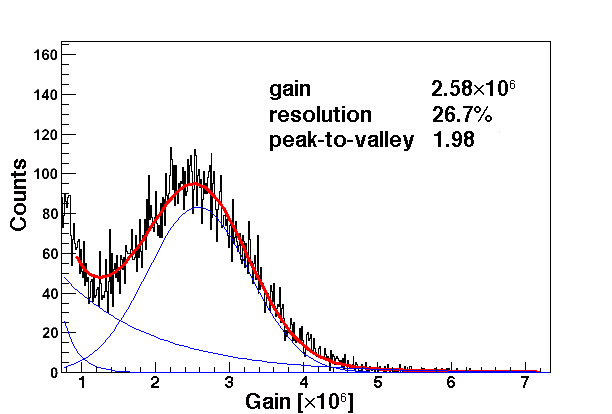
\includegraphics[width=0.475\linewidth]{plots/PMTtest/GoodPMTspectrum1.png}
\label{figPMTtestSER_1}}
\subfigure[]{
%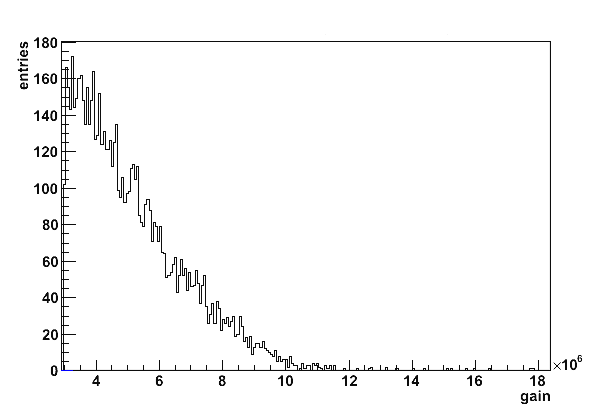
\includegraphics[width=0.475\linewidth]{plots/PMTtest/PMTtest_BadPMT.png}
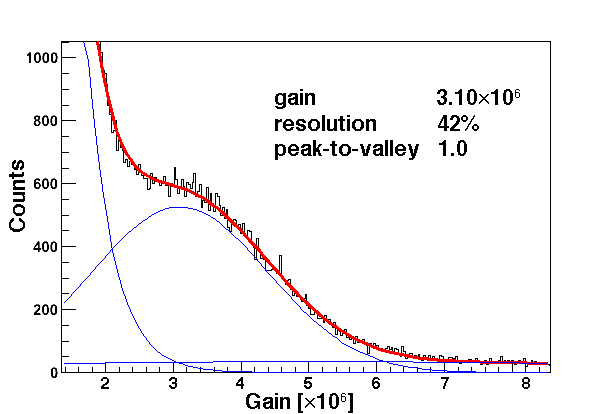
\includegraphics[width=0.475\linewidth]{plots/PMTtest/BadPMTspectrum1.png}
\label{figPMTtestSER_2}}
\caption[Single photoelectron response of the R8520 Hamamatsu phototubes, measured in the room temperature]{Single photoelectron response of the R8520 Hamamatsu phototubes, measured in the room temperature: (a) - typical single PE spectrum of a PMT chosen to be used in XENON100; (b) - response of the PMT not used in the experiment due to low peak-to-valley ratio, and hence bad separation between noise and signal.}
%PMT with a bad single PE response, peak-to-valley ratio around 1, not used in the experiment.}
\label{figPMTtestSER}
\end{figure}

The gain has been measured with a different high voltage supplied to each PMT (Fig.~\ref{figGainVShv_1}). The current amplification increases proportional to the exponential power of the supply voltage:

\begin{equation}
\mathrm{gain} = A \cdot V^{kn},
\end{equation} 
where $A$ is a constant, $V$ - supply voltage, $n$ - number of dynodes, and $k$ - constant determined by the structure and material of the electrodes. 
The single PE resolution becomes improves with an increase of PMT gain, as shown in Fig.~\ref{figGainVShv_2}.

\begin{figure}[!t]
\centering
\subfigure[]{
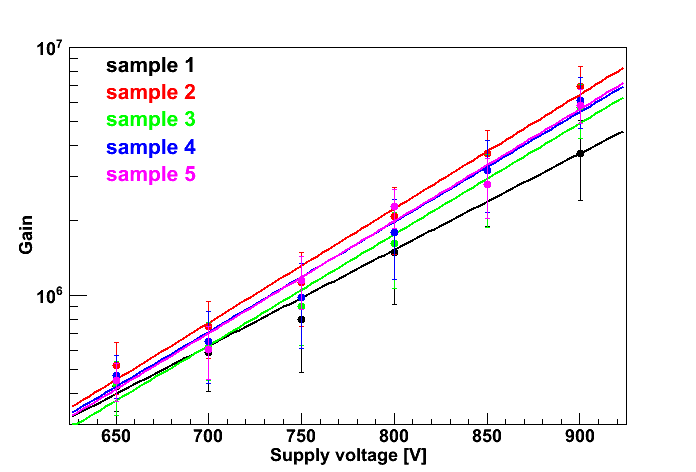
\includegraphics[width=0.475\linewidth]{plots/PMTtest/gainVShv.png}
\label{figGainVShv_1}}
\subfigure[]{
%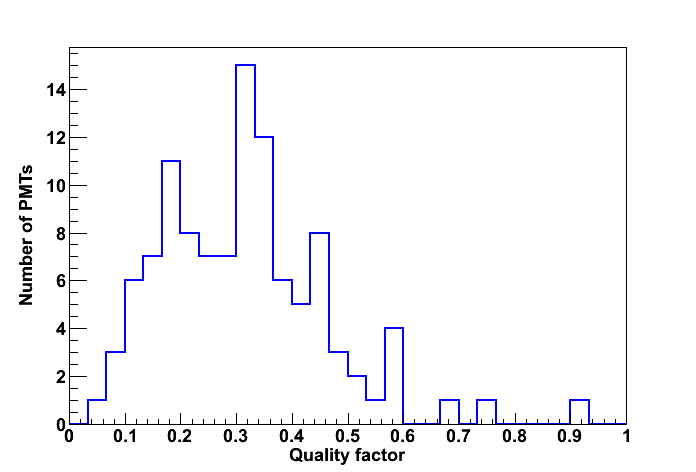
\includegraphics[width=0.475\linewidth]{plots/PMTtest/QualityFactor.png}
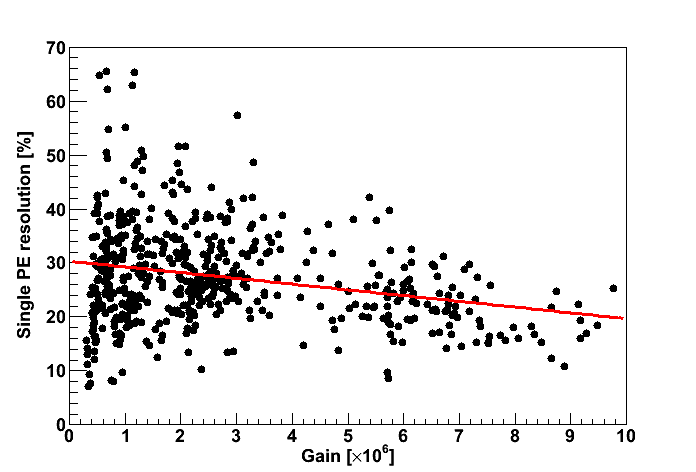
\includegraphics[width=0.475\linewidth]{plots/PMTtest/resVSgain.png}
\label{figGainVShv_2}}
\caption[Measured PMT gain as a function of the supply voltage and the correlation between single photoelectron resolution and  gain]{Measured PMT gain as a function of the supply voltage (a), and correlation between the single photoelectron resolution and the gain (b).}

% and the quality factor, defined as the ratio of the peak-to-valley ratio and the single photoelectron resolution, which correspond to PMT gain of $\sim$2$\times$10$^{6}$.}
\label{figGainVShv}
\end{figure}


No major changes have been observed between the low QE and high QE batches of PMTs in the mean values of peak-to-valley ratio and single PE resolution. However, as shown in Fig.~\ref{figPMTtestCorrelation_2}, the average gain of low QE PMTs is almost twice higher than that of the high QE ones, measured at the same supply voltage. This effect is also present within the PMTs of the same batch: there is a  correlation between the measured gain at fixed voltage and QE, provided by the manufacturer for each PMT. It is indicated with a thick blue line in Fig.~\ref{figPMTtestCorrelation_2}. This anti-correlation between QE and gain parameters could not be explained, and might be a product of the systematics of the spectral response measurements performed by the manufacturer.

%\begin{figure}[!h]
%\centering
%\subfigure[]{
%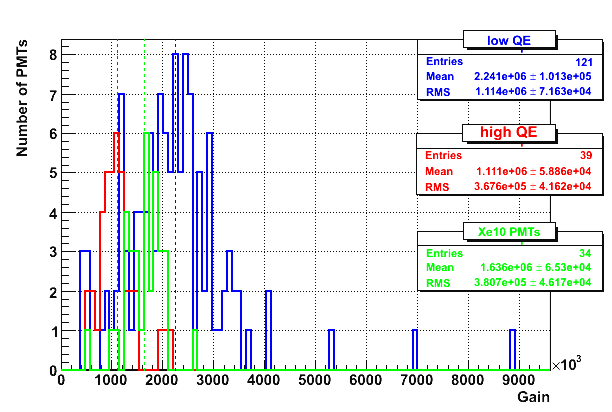
\includegraphics[width=0.475\linewidth]{plots/PMTtest/lowQE_highQE_xe10_GAIN.png}
%\label{figPMTtestResults_1}}
%\subfigure[]{
%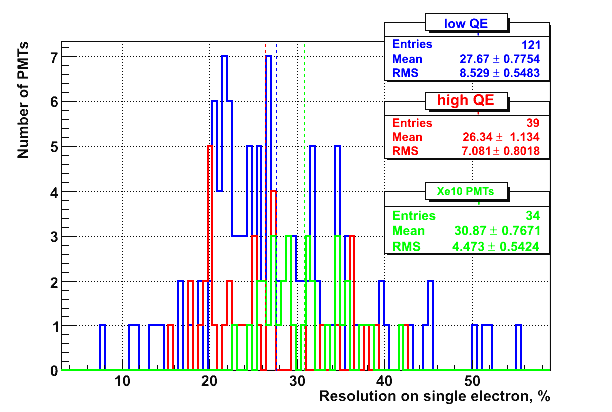
\includegraphics[width=0.475\linewidth]{plots/PMTtest/lowQE_highQE_xe10_RES.png}
%\label{figPMTtestResults_2}}
%\subfigure[]{
%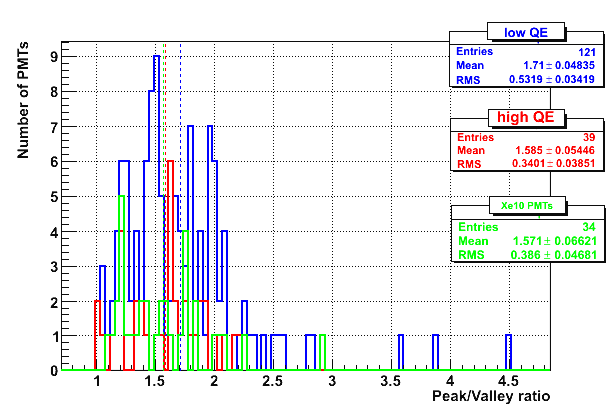
\includegraphics[width=0.3\linewidth]{plots/PMTtest/lowQE_highQE_xe10_PV.png}
%\label{figPMTtestResults_3}}
%\caption[Results of the PMT tests in room temperature for different PMT batches]{Results of the PMT tests in room temperature for different PMT batches: (a) - gain at fixed supply voltage of 900~V, (b) - resolution on single PE.
%, (c) - peak-to-valley ratio.
%}
%\label{figPMTtestResults}
%\end{figure}


\begin{figure}[!h]
\centering
\subfigure[]{
%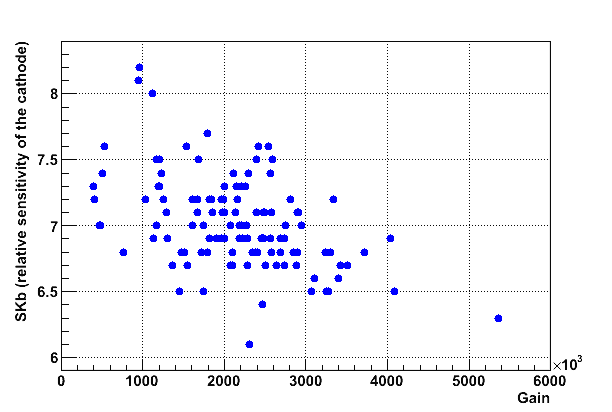
\includegraphics[width=0.475\linewidth]{plots/PMTtest/122lowQE_SKBvsGAIN_zoom.png}
%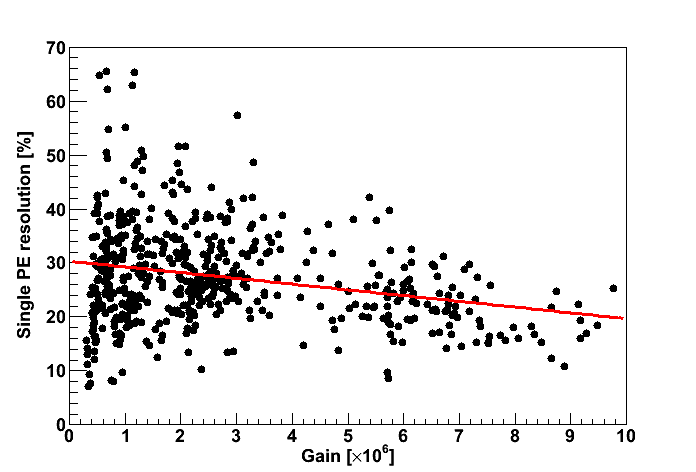
\includegraphics[width=0.475\linewidth]{plots/PMTtest/resVSgain.png}
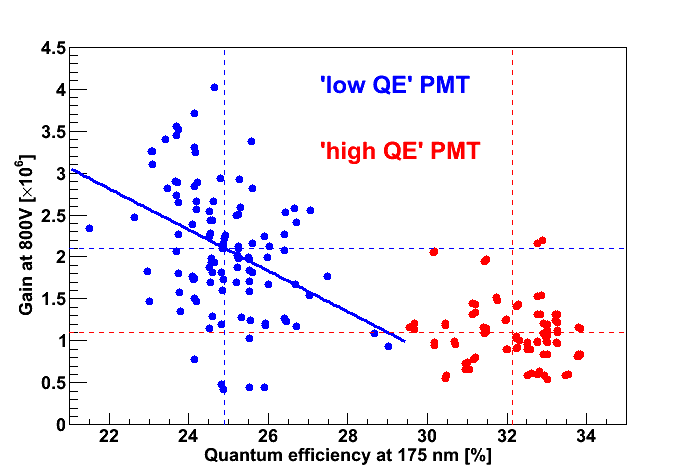
\includegraphics[width=0.475\linewidth]{plots/PMTtest/gainVSqe_LowHigh_withLines.png}
\label{figPMTtestCorrelation_1}}
\subfigure[]{
%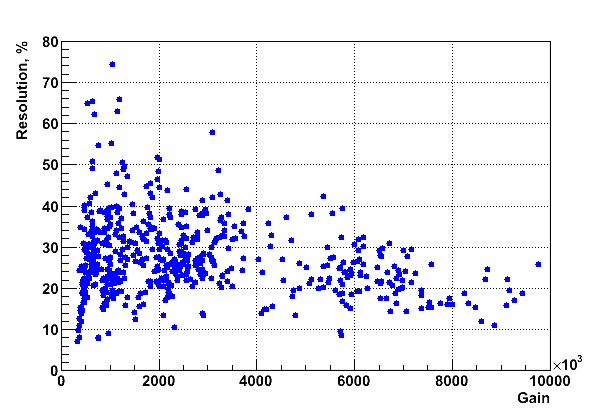
\includegraphics[width=0.475\linewidth]{plots/PMTtest/122lowQE_resVSgain.png}
%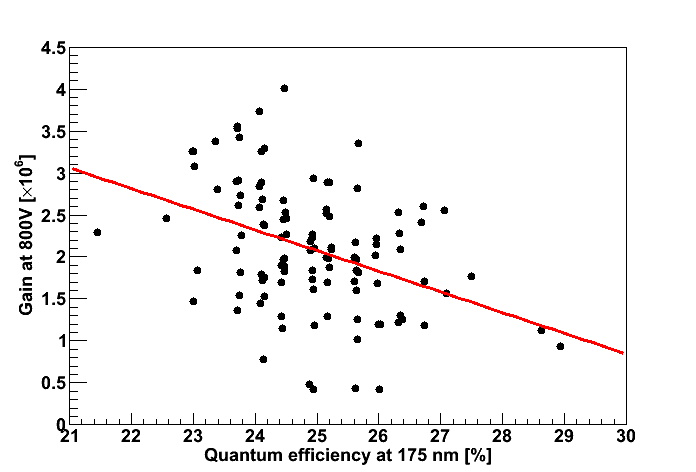
\includegraphics[width=0.475\linewidth]{plots/PMTtest/gainVSqe.png}
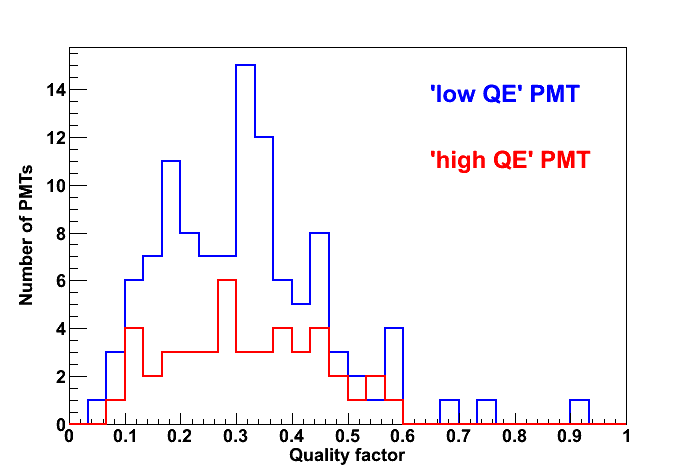
\includegraphics[width=0.475\linewidth]{plots/PMTtest/QualityFactor_LowHigh.png}
\label{figPMTtestCorrelation_2}}
\caption[Correlation between the PMT gain measured at fixed voltage and quantum efficiency provided by the manufacturer, and the PMT test quality factor]{(a) - correlation between the PMT gain measured at fixed voltage (800~V) and quantum efficiency (QE) provided by the manufacturer. The vertical and horizontal dashed lines show the average gain and QE, respectively. The thick blue line is a fit to the low QE PMTs data points. (b) - the quality factor, defined as the ratio of the peak-to-valley ratio and the single photoelectron resolution, which correspond to PMT gain of $\sim$2$\times$10$^{6}$.}
\label{figPMTtestCorrelation}
\end{figure}

In addition to the measurement of PMT characteristics, all high QE phototubes have been tested to withstand the thermal shocks from room to cryogenic temperature using dry ice (solid carbon dioxide, temperature $-$78.5$^{\circ}$C). This has been necessary, as these PMTs have been produced specifically for XENON100 using a new type of vacuum sealing, and potential problems have been reported by the manufacturer. Out of the 58 PMTs that have undergone the cooling test, 10 PMTs showed problems (discharge while raising the supply voltage or absence of signal), and have been returned to the factory for a replacement.

For all PMTs classified as working after the tests, a `quality factor' has been defined as the ratio of the measured peak-to-valley ratio and resolution on single PE. The distribution of this parameter is shown in Fig.~\ref{figPMTtestCorrelation_2} and centered around 0.3 for both low QE and high QE PMT batches. In addition to QE, this quality factor has been used to compare the PMTs and distribute them within the different arrays in the detector. All high QE PMTs have been placed on the bottom array in the target volume to ensure that the detected light yield (S1) is as high as possible. The phototubes with the highest QE have been placed in the center of the array. The `low QE' PMTs have been placed on the top array in the target volume in the veto.



